%
% Niniejszy plik stanowi przykład formatowania pracy magisterskiej na
% Wydziale MIM UW.  Szkielet użytych poleceń można wykorzystywać do
% woli, np. formatujac wlasna prace.
%
% Zawartosc merytoryczna stanowi oryginalnosiagniecie
% naukowosciowe Marcina Wolinskiego.  Wszelkie prawa zastrzeżone.
%
% Copyright (c) 2001 by Marcin Woliński <M.Wolinski@gust.org.pl>
% Poprawki spowodowane zmianami przepisów - Marcin Szczuka, 1.10.2004
% Poprawki spowodowane zmianami przepisow i ujednolicenie 
% - Seweryn Karłowicz, 05.05.2006
% Dodanie wielu autorów i tłumaczenia na angielski - Kuba Pochrybniak, 29.11.2016

% dodaj opcję [licencjacka] dla pracy licencjackiej
% dodaj opcję [en] dla wersji angielskiej (mogą być obie: [licencjacka,en])
\documentclass[licencjacka]{pracamgr}


% Dane magistranta:
\autor{Michał Izworski}{360968}


% Dane magistrantów:
%\autor{Autor Zerowy}{342007}
%\autori{Autor Pierwszy}{342013}
%\autorii{Drugi Autor-Z-Rzędu}{231023}
%\autoriii{Trzeci z Autorów}{777321}
%\autoriv{Autor nr Cztery}{432145}
%\autorv{Autor nr Pięć}{342011}

\title{AlphaSoccer: gra w ,,Piłkarzyki~na~kartce'' za pomocą głębokich sieci neuronowych}


%\tytulang{An implementation of a difference blabalizer based on the theory of $\sigma$ -- $\rho$ phetors}

%kierunek: 
% - matematyka, informacyka, ...
% - Mathematics, Computer Science, ...
\kierunek{Międzykierunkowe Studia Ekonomiczno-Matematyczne}

% informatyka - nie okreslamy zakresu (opcja zakomentowana)
% matematyka - zakres moze pozostac nieokreslony,
% a jesli ma byc okreslony dla pracy mgr,
% to przyjmuje jedna z wartosci:
% {metod matematycznych w finansach}
% {metod matematycznych w ubezpieczeniach}
% {matematyki stosowanej}
% {nauczania matematyki}
% Dla pracy licencjackiej mamy natomiast
% mozliwosc wpisania takiej wartosci zakresu:
% {Jednoczesnych Studiow Ekonomiczno--Matematycznych}

% \zakres{Tu wpisac, jesli trzeba, jedna z opcji podanych wyzej}

% Praca wykonana pod kierunkiem:
% (podać tytuł/stopień imię i nazwisko opiekuna
% Instytut
% ew. Wydział ew. Uczelnia (jeżeli nie MIM UW))
\opiekun{prof. dr hab. Andrzej Skowron\\
  Wydział Matematyki, Informatyki i Mechaniki\\
  }

% miesiąc i~rok:
\date{Czerwiec 2018}

%Podać dziedzinę wg klasyfikacji Socrates-Erasmus:
\dziedzina{ 
%11.0 Matematyka, Informatyka:\\ 
%11.1 Matematyka\\ 
%11.2 Statystyka\\ 
%11.3 Informatyka\\ 
11.4 Sztuczna inteligencja\\ 
%11.5 Nauki aktuarialne\\
%11.9 Inne nauki matematyczne i informatyczne
}

%Klasyfikacja tematyczna wedlug AMS (matematyka) lub ACM (informatyka)
\klasyfikacja{Computing methodologies\\
	Machine learning\\
 	Learning paradigms\\
	Reinforcement learning\\
	Sequential decision making}

% Słowa kluczowe:
\keywords{machine learning, reinforcement learning, deep learning, actor-critic methods, monte carlo tree search}

% Tu jest dobre miejsce na Twoje własne makra i~środowiska:
\newtheorem{defi}{Definicja}[section]
\usepackage{wrapfig}
\usepackage{graphicx}
\graphicspath{ {img/} }
\usepackage{algorithm}
\usepackage[noend]{algpseudocode}
\usepackage{amsmath,amsfonts}

\makeatletter
\def\BState{\State\hskip-\ALG@thistlm}
\makeatother

% koniec definicji

\begin{document}

\maketitle

%tu idzie streszczenie na strone poczatkowa
\begin{abstract}
  TO DO
\end{abstract}

\tableofcontents
%\listoffigures
%\listoftables

\chapter{Wprowadzenie}\label{r:intro}

%Sztuczna inteligencja cieszy się ogromnym wzrostem zainteresowania w ostatnim czasie, zarówno wśród społeczności naukowej, jak i w przemyśle. Swoją popularność zawdzięcza temu, iż dzięki niej jesteśmy w stanie poradzić sobie z problemami, których rozwiązania przy użyciu programów komputerowych przynosiły bardzo mierne rezultaty. 
%Na szczególną uwagę zasługuje Uczenie Maszynowe (ang. Machine Learning), które jest obecnie wiodącym nurtem i przyciąga największą uwagę ze względu na najlepsze rezultaty.
%Pozwoliło nam ono na tworzenie programów do rozpoznawania obrazów, tłumaczenia maszynowego czy generowania muzyki. 
%Sztuczna inteligencja okazała się 

%Uczenie Maszynowe cieszy się ogromnym wzrostem zainteresowania w ostatnim czasie, zarówno wśród społeczności naukowej, jak i w przemyśle.
%Pozwoliło nam ono na rozwiązanie problemów, których wcześniejsze próby rozwiązania dawały kiepskie rezultaty, takich jak rozpoznawania obrazów, tłumaczenia maszynowego czy generowania muzyki.
%Jednym z przełomowych wyników sztucznej inteligencji, jakie udało nam się uzyskać

%\section{Intro}

Interakcja z otoczeniem jest prawdopodobnie dla większości z nas naturalnym sposobem uczenia się. 
Dziecko uczące się stawiać pierwsze kroki nie posiada nauczyciela, który dokładnie instruuje je w jaki sposób powinno układać nogi, aby zachować równowagę. 
Zamiast tego, poprzez metodę prób i błędów, stara się ono zrozumieć w jaki sposób zrealizować swój cel i poznaje jakie efekty przynosi wykonywanie przez nie konkretnych ruchów. 
W ten sam sposób uczymy się przez całe życie, jednocześnie poznając otaczający nas świat oraz prawa, które nim rządzą, bez względu na to czy jest to nauka jazdy samochodem czy gry w szachy.

%\section{Intro2}

\section{Piłkarzyki na kartce}

Piłkarzyki na kartce to gra strategiczna, odbywającą się na prostokątnym boisku, rysowanym zazwyczaj na kartce w kratę.
Gracze na przemian wykonują ruchy polegające na przemieszczeniu piłki na sąsiednie pola, aż znajdzie się ona w jednej z bramek lub nie będzie możliwe wykonanie kolejnego ruchu.

\begin{figure}[ht]
  \centering
  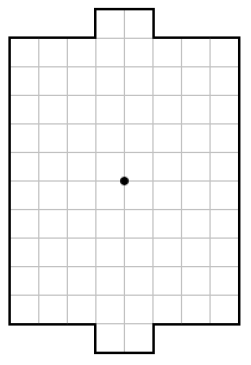
\includegraphics[width=0.2\textwidth]{board}
  \caption{Pusta plansza}
\end{figure}

Najczęściej stosowanym wymiarem planszy jest 8x10 kratek.
Przy krótszych bokach narysowane są dwie bramki o szerokości 2 kratek, w których gracze muszą umieścić piłkę.
Rozgrywka toczy się jedynie na przecięciach linii.
Środek planszy jest punktem startowym gry, do którego gracze dorysowują kolejne linie, oznaczające przemieszczenie piłki na sąsiednie pole. Każdy kolejny ruch zaczyna się w miejscu, w którym skończył się poprzedni, wzdłuż kratki lub po przekątnej. 

Ruchy nie mogą odbywać się po brzegu planszy ani wzdłuż odcinków, po których wcześniej piłka była już prowadzona.
Możliwe jest odbijanie się, które polega na wykonaniu przez gracza dodatkowego ruchu. Następuje ono gdy ruch zostanie zakończony w miejscu, w którym kończy się już linia narysowana przez jednego z graczy lub na brzegu boiska. 

\begin{figure}[ht]
  \centering
  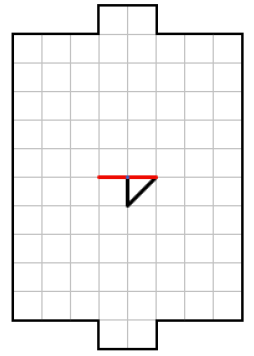
\includegraphics[width=0.2\textwidth]{odbicie}
  \caption{Odbicie (kolor czerwony)}
\end{figure}

Gra kończy się w momencie gdy piłka znajdzie się w jednej z bramek.
Wówczas gracz, do którego należy dana bramka, przegrywa. 
Gracz może również przegrać w wypadku gdy nie jest w stanie wykonać żadnego ruchu.


\begin{figure}[ht]
  \centering
  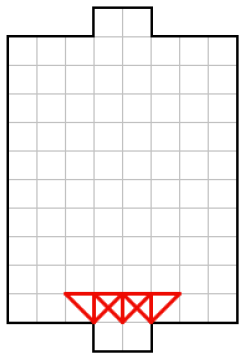
\includegraphics[width=0.2\textwidth]{zablokowanie}
  \caption{Zablokowana bramka}
\end{figure}
 
\section{Cel badawczy} 

% todo napisz wczesniej cos o AlphaGo

Celem mojej pracy jest zastosowanie algorytmu wykorzystanego w AlpaGo, do wyuczenia agenta zdolnego do gry w piłkarzyki na kartce. Postaram się w niej dowiedzieć w jaki sposób hiperparametry wykorzystane w AlphaGo powinny zostać zaadaptowane do mojego problemu. 

Ponadto maszyny wykorzystywane podczas uczenia AlphaGo są rzędy wielkości większe od typowych komputerów, które są dostępne dla przeciętnego studenta. Moje eksperymenty będą skupiały się również na tym jak hiperparametry modelu mogą być redukowane, aby jednocześnie uzyskać wyniki w sensownym czasie oraz aby były one dla nas satysfakcjonujące.


\section{Wkład własny}

Za mój wkład uważam:

\begin{itemize}

\item Zastosowanie metod uczenia ze wzmocnieniem do piłkarzyków na papierze, które wcześniej nie przyciągnęły wcześniej niczyjej uwagi,

\item Implementacja algorytmu AlphaGo, którego dostępny jest jedynie opis słowny,

\item Wyznaczenie które hiperparametry mogą zostać zredukowane, aby móc przeprowadzić eksperyment na przeciętnej maszynie oraz wyznaczenie tych hiperparametrów, które zostały pominięte w pracy AlphaGo.

\end{itemize}

\section{Zarys pracy}

Pozostała część pracy została podzielona na następujące rozdziały:

W rozdziale drugim postaram wprowadzić czytelnika w zagadnienie uczenia ze wzmocnieniem, wyprowadzając podstawowe definicje oraz pojęcia, które wykorzystywane będą w późniejszych rozdziałach pracy.

W rozdziale trzecim zaznajomię czytelnika z tematem głębokich sieci neuronowych, które stanowią dziś ogromną część uczenia maszynowego i cieszą się ogromną popularnością ze względu na swoje znakomite osiągnięcia.

W rozdziale czwartym wytłumaczę w jaki sposób połączyć ze sobą światy uczenia ze wzmocnieniem oraz głębokich sieci neuronowych, otrzymując w ten sposób głębokie uczenie ze wzmocnieniem, które odpowiedzialne jest obecnie za czołowe osiągnięcie w dziedzinie uczenia ze wzmocnieniem, takie jak autonomiczne samochody czy AlphaGo.

W rozdziale piątym opowiem o wykonanym przeze mnie eksperymencie uczenia się gry w piłkarzyki na kartce. Wyjaśnię w jaki sposób algorytm zdobywa doświadczenie potrzebne mu podczas uczenia się oraz w jaki sposób wygląda proces podejmowania decyzji oraz uczenia się.

Ostatni rozdział podsumowuje wykonaną pracę i zawiera moje wnioski wyciągnięte podczas tej pracy.
 
\chapter{Uczenie ze Wzmocnieniem}\label{r:rl}

\section{Wprowadzenie}

Uczenie ze wzmocnieniem (ang. Reinforcement Learning, RL) jest działem uczenia maszynowego, zajmującym się sekwencyjnym podejmowaniem decyzji. Na proces uczenia składa się \emph{agent}, który uczy się podejmować decyzje oraz \emph{środowisko}, które stanowi cały świat zewnętrzy dla agenta. Interakcja między nimi polega na naprzemiennym wykonywaniu akcji przez agenta oraz prezentowaniu nowej sytuacji, w której on się znalazł i nagrody jaką otrzymał przez środowisko. Celem agenta jest maksymalizacja nagród, które otrzymuje.
Podczas procesu uczenia się, nigdy nie wskazujemy agentowi którą akcje powinien on wykonać, co stanowi główną różnice pomiędzy uczeniem ze wzmocnieniem a uczeniem nadzorowanym (ang. Supervised Learning). 

\section{Dyskretny Proces Markowa}

Dyskretny Proces Markowa składa się z:
\begin{itemize}
\item zbioru stanów w których może znaleźć się agent, $ s \in \mathcal{S} $,
\item rozkładu stanu początkowego $\mathcal{D}$ nad zbiorem $\mathcal{S}$,
\item zbioru akcji możliwych do podjęcia przez agenta, $ a \in \mathcal{A} $
\item nagrody otrzymywanej przez agenta za każdym razem, gdy ten wykona jakąś akcje, $ r_t \in \mathbb{R} $
\item prawdopodobieństwa przejścia między stanami
$$ p(s'|s, a) = \mathbb{P}(s_{t+1} = s' \mid s_t = s, a_t = a)$$
\item funkcji nagrody, $ R : S \times S \times A \rightarrow \mathbb{R} $
$$ R(s, a, s') = \mathbb{E}(r_{t+1} \mid s_t = s, a_t = a, s_{t+1} = s') $$
\item współczynnik dyskontującego wartości nagród otrzymywanych w przyszłości $ \gamma \in [0, 1] $
\end{itemize}


\section{Wynik oraz epizody}

Interakcja między agentem a środowiskiem zachodzi w każdym, dyskretnym punkcie czasu $ t = 0, 1, 2, ... $. Znajdując się w punkcie czasu $t$, agent obserwuje stan $ s_t \in \mathcal{S} $, w którym się znajduję, na jego podstawie wykonuje akcję $ a_t \in \mathcal{A}(s) $, gdzie $ \mathcal{A}(s) $ jest zbiorem wszystkich akcji, które można wykonać znajdując się w stanie $s$. W kolejnym kroku dowiaduje się on jaką nagrodę $ r_{t+1} \in \mathbb{R} $ otrzymał i do jakiego stanu $ s_t{t+1} $ się przeniósł. W wyniku otrzymujemy następujący ciąg stanów, akcji oraz nagród, zwany \emph{trajektorią}:

$$ s_0, a_0, r_1, s_1, a_1, r_2, ... $$


\begin{figure}[ht]
  \centering
  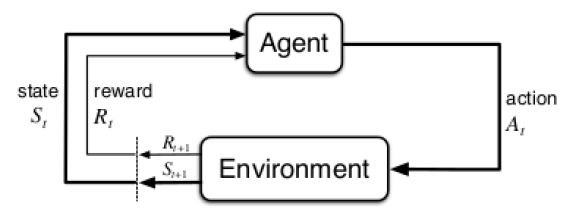
\includegraphics[width=0.5\textwidth]{agent_env_interaction}
  \caption{Interakcja między agentem a środowiskiem jako Dyskretny Proces Markowa}
\end{figure}

Najprostszym typem środowisk są te w których ilość kroków jest z góry ograniczona. Pojedynczy ciąg interakcji nazywamy wówczas \emph{epizodem}, a ostatni stan obserwowany przez agenta -- \emph{stanem terminalnym}. W tym wypadku epizody są od siebie niezależne, mogą się one kończyć w różnych stanach oraz po różnej ilości kroków. 

Celem naszego agenta jest maksymalizacja wartości oczekiwanej sumy nagród, które zdobędzie on w przyszłości. Określmy ją jako \emph{wynik}, $ G_t $, który zdefiniowany jest następująco:

$$ G_t = r_{t+1} + r_{t+2} + r_{t+3} + ... + r_{T-1} = r_{t+1} + G_{t+1} $$

gdzie $T$ jest końcem epizodu, a $t$ indeksem czasu. Sam problem nauczenia naszego agenta w jaki sposób powinien on podejmować decyzje, aby osiągnąć najwyższy wynik, nazywamy \emph{epizodycznym zadaniem}.

Możemy również spotkać się ze środowiskami, z którymi interakcja przebiega nieprzerwanie. Mamy wówczas do czynienia z \emph{ciągłym zadaniem}. Wprowadzamy wówczas koncepcje \emph{dyskontowania} wyniku, który definiujemy następująco:

$$ G_t = r_{t+1} + \gamma r_{t+2} + \gamma^2 r_{t+3} + ... = 
\sum_{k=0}^{\infty} \gamma^k r_{t+k+1} $$

gdzie $ \gamma \in [0, 1) $.


\section{Polityka}

Polityka jest funkcją która każdemu stanowi przyporządkowuje akcję. Może być ona deterministyczna, $ \pi(s) $, bądź też stochastyczna, $ \pi(a \mid s) $, i wówczas stanowić rozkład prawdopodobieństwa wszystkich akcji dla ustalonego stanu. Metody uczenia ze wzmocnieniem określają w jaki sposób polityka jest modyfikowana na podstawie doświadczenia zbieranego przez agenta.

\section{Funkcja Wartości}

Posiadając już politykę naszego agenta, możemy chcieć się dowiedzieć jaką nagrodę uzyska agent, który będzie jej przestrzegał. W tym celu definiujemy \emph{funkcję wartości stanu} (ang. Value Function), którą oznaczamy jako $ v_{\pi}(s) $ dla ustalonej polityki $ \pi $. Definiujemy ją jako:

$$ v_{\pi}(s) = \mathbb{E}_{\pi}[G_t \mid S_t = s] = \mathbb{E}_{\pi} \Bigg[ \sum_{k=0}^{\infty} \gamma^k R_{t+k+1} \bigg| S_t = s \Bigg] $$

gdzie $ \mathbb{E}_{\pi} $ jest wartością oczekiwaną przy założeniu że agent kieruje się polityką $\pi$, z kolei $t$ jest dowolnym punktem w czasie. 

Podobnie definiujemy wartość wybrania akcji $a$, gdy znajdujemy się w stanie $s$ oraz podążamy zgodnie z polityką $\pi$, oznaczaną jako $q_{\pi}(s, a)$. Jest ona wartością oczekiwaną z sytuacji w której rozpoczynamy w stanie $s$, wykonujemy akcję $a$, po czym wszystkie kolejne akcje wykonujemy zgodnie z polityką $\pi$. Funkcję tę nazywamy \emph{funkcją wartości akcji} lub \emph{Q-funkcją}.

$$ q_{\pi}(s, a) = \mathbb{E}_{\pi}[G_t \mid S_t = s, A_t = a] = \mathbb{E}_{\pi} \Bigg[ \sum_{k=0}^{\infty} \gamma^k R_{t+k+1} \bigg| S_t = s, A_t = a \Bigg] $$

\section{Optymalność polityki oraz funkcji wartości}

Podczas rozwiązywania problemu uczenia ze wzmocnieniem staramy się znaleźć politykę, której przestrzeganie przyniesie naszemu agentowi jak największą nagrodę. Będziemy mówić że polityka $\pi$ jest lepsza lub równa polityce $\pi'$, wtedy i tylko wtedy gdy oczekiwana nagroda dla niej jest większa lub równa niż dla $\pi'$ w każdym stanie należącym do przestrzeni stanów. Zawsze istnieje polityka, która jest lepsza lub równa od wszystkich innych i nazywamy ją \emph{optymalną polityką}. Może istnieć wiele różnych od siebie optymalnych polityk, jednak każdą z nich oznaczamy jako $\pi_{\ast}$. Dla wszystkich z nich funkcja wartości stanu jest taka sama i nazywamy ją \emph{optymalną funkcją wartości stanu}. Spełnia ona własność:

$$ v_{\ast}(s) = \max_{\pi} v_{\pi}(s) $$

dla każdego stanu $s \in \mathcal{S}$. Podobnie współdzielą one \emph{optymalną funkcję wartości akcji}, $q_{\ast}$, która spełnia:

$$ q_{\ast}(s, a) = \max_{\pi} q_{\pi}(s, a) $$

dla każdego stanu $s \in \mathcal{S}$ oraz akcji $a \in \mathcal{A}$.

Ponadto optymalną funkcję wartości stanu możemy zdefiniować odwołując się do funkcji wartości akcji w następujący sposób:

$$ v_{\ast}(s) = \max_{a \in \mathcal{A}} q_{\pi_{\ast}}(s) $$

Podstawową własnością, jaką spełniają funkcje wartości, jest \emph{równanie Bellmana}. Dla dowolnej polityki $\pi$ oraz stanu $s$ zachodzi:

\begin{align}
v_{\pi}(s) &= \mathbb{E}_{\pi}[G_t \mid S_t = s]  \nonumber \\
&= \mathbb{E}_{\pi}[r_{t+1} + \gamma G_{t+1} \mid S_t = s] \nonumber \\
&= \sum_a \pi(a \mid s) \sum_s' \sum_r p(s', r \mid s, a) \Big[r + \gamma \mathbb{E}_{\pi}[G_{t+1} \mid S_{t+1} = s' ]\Big] \nonumber \\
&= \sum_a \pi(a \mid s) \sum_{s', r} p(s', r \mid s, a) \Big[r + \gamma v_{\pi}(s') \Big]
\end{align}

Na podstawie własności optymalnych funkcji wartości oraz równania Bellmana możemy wyprowadzić \emph{równania optymalności Bellmana}, bez odwoływania się przy tym do żadnej polityki. Pierwsze z nich odnosi się do funkcji wartości stanu:

\begin{align}
v_{\ast}(s) &= \max_{a \in \mathcal{A}} q_{\pi_{\ast}}(s, a) \nonumber \\
&= \max_a \mathbb{E}_{\pi}[G_t \mid S_t = s, A_t = a]  \nonumber \\
&= \max_a \mathbb{E}_{\pi}[r_{t+1} + \gamma G_{t+1} \mid S_t = s, A_t = a] \nonumber \\
&= \max_a \mathbb{E}[r_{t+1} + \gamma v_{\pi_{\ast}}(S_{t+1}) \mid S_t = s, A_t = a] \nonumber \\
&= \max_a \sum_{s', r} p(s', r \mid s, a) \Big[r + \gamma v_{\ast}(s') \Big]
\end{align}

Natomiast drugie zdefiniowane jest dla funkcji wartości akcji:

\begin{align}
q_{\ast}(s, a) &= \mathbb{E}[r_{t+1} + \gamma \max_{a'} q_{\ast} (S_{t+1}, a') \mid S_t = s, A_t = a] \nonumber \\
&= \sum_{s', r} p(s', r \mid s, a) \Big[r + \gamma \max_{a'} q_{\ast} (s', a') \Big]
\end{align}

\section{Metody uczenia ze wzmocnieniem}

Metody rozwiązywania problemu uczenia ze wzmocnieniem możemy podzielić ze względu na to, czy wykorzystują one model środowiska. Metody \emph{model-based} wymagają od nas \emph{modelu} środowiska, z którego nasz agent będzie korzystał podczas aby przewidzieć w jaki sposób środowisko będzie zachowywało się w odpowiedzi na wykonywane przez niego akcje.
Dzięki temu możliwe jest \emph{planowanie}, które pozwala na przewidywanie zachowania środowiska wiele kroków wprzód. Tego typu problemy możemy spotkać przy okazji nauki naszego agenta w Go, gdzie środowisko imitowane jest przez niego samego, podczas gdy gra on sam ze sobą. 
Drugą klasą algorytmów są metody \emph{model-free}, w których agent posiada jedynie politykę oraz funkcję wartości, a samo zachowanie środowiska jest dla niego nieznane i może on obserwować jedynie bezpośrednie skutki swoich działań. Z takimi problemami spotykamy się np. w przypadku gry naszego agenta na Atari, gdzie nie próbujemy dowiedzieć się jakie prawa rządzą poszczególnymi grami, a zamiast tego po prostu dajemy naszemu agentowi grać.

\subsection{Metody Monte Carlo}

Metody Monte Carlo korzystają z idei \emph{uogólnionej iteracji polityki}, która składa się z dwóch, przeplatających się ze sobą procesów. Pierwszy krok, nazywany \emph{krokiem ewaluacji polityki}, polega na aproksymacji funkcji wartości na podstawie polityki, wykorzystywanej przez agenta. Z kolei w drugim kroku ulepszamy obecną politykę, przy użyciu wcześniej uzyskanej funkcji wartości. Nazywamy go \emph{krokiem ulepszania polityki}.

W przypadku metod Monte Carlo, ewaluacje polityki wykonujemy poprzez próbkowanie kolejnych trajektorii, a następnie wyliczanie średniego wyniku dla każdego ze stanów, bądź każdej pary stan-akcja. Zbierana przez nas historia akcji w postaci trajektorii nazywamy \emph{doświadczeniem} agenta. Najprostszy sposób aktualizacji funkcji wartości może wyglądać następująco:

$$ v(s_t) \leftarrow v(s_t) + \alpha \big[G_t - v(s_t)\big] $$

gdzie $G_t$ oznacza wynik agenta następujący po czasie $t$, a $\alpha$ parametrem wpływającym na szybkość uczenia się.

Ulepszanie polityki następuje poprzez zachłanny wybór najlepszej akcji dla każdego ze stanów, przy pomocy funkcji wartości akcji. Jednak w przypadku takiego doboru polityki, skazujemy się na deterministyczną politykę, która nie jest w stanie odkrywać nowych, potencjalnie lepszych akcji, gdyż cały czas wybierać będzie ona te same akcje. 

Aby utrzymać eksploracje nowych akcji oraz stanów, wprowadzamy pojęcie \emph{$\epsilon$--zachłannej} polityki, która z wysokim prawdopodobieństwem wykonuje akcję, która maksymalizuje wartość funkcji wartości akcji, a od czasu do czasu wykonuje losową akcję. Dzięki temu utrzymujemy stały poziom eksploracji, a przy niewielkich założeniach dla epsilona polityka zbiega do optymalnej.

$$
\pi(a \mid s) =
\begin{cases}
    1 - \epsilon + \epsilon/\lvert \mathcal{A}(s) \rvert & \text{if } a = a^\ast \\
    \epsilon/\lvert \mathcal{A}(s) \rvert,              & \text{if } a\neq a^\ast
\end{cases}
$$

Metody Monte Carlo cierpią z powodu wysokiej wariancji podczas uczenia, przez co potrzeba bardzo wielu iteracji, aby agent mógł wyuczyć się sensownej polityki. Są one przykładem metod model-free.

\subsection{Temporal-Difference Learning} 

Prawdopodobnie najważniejszą ideą wykorzystywaną  w uczeniu ze wzmocnieniem jest \emph{temporal-difference} (TD) learning. Podobnie do metod Monte Carlo wykorzystuje ono doświadczenie agenta, bez użycia modelu środowiska. Nie jest wymagane jednak oczekiwanie na zakończenie epizodu, aby zaktualizować wartość funkcji wartości, a zamiast tego aktualizacje mogą następować po wykonaniu pojedynczego kroku. Aktualizacja funkcji wartości w przypadku TD learning może wyglądać następująco:

$$ V(S_t) \leftarrow V(S_t) + \alpha \big[R_{t+1} + \gamma V(S_{t+1}) - V(S_t) \big] $$

Sposób tej aktualizacji nazywany jest \emph{TD(0)} lub też \emph{jedno--krokowym} TD, a sam wyraz o który aktualizowana jest wartość:

$$ \delta_t = R_{t+1} + \gamma V(S_{t+1}) - V(S_t) $$

nazywamy \emph{błędem TD}.

\begin{figure}[ht]
  \centering
  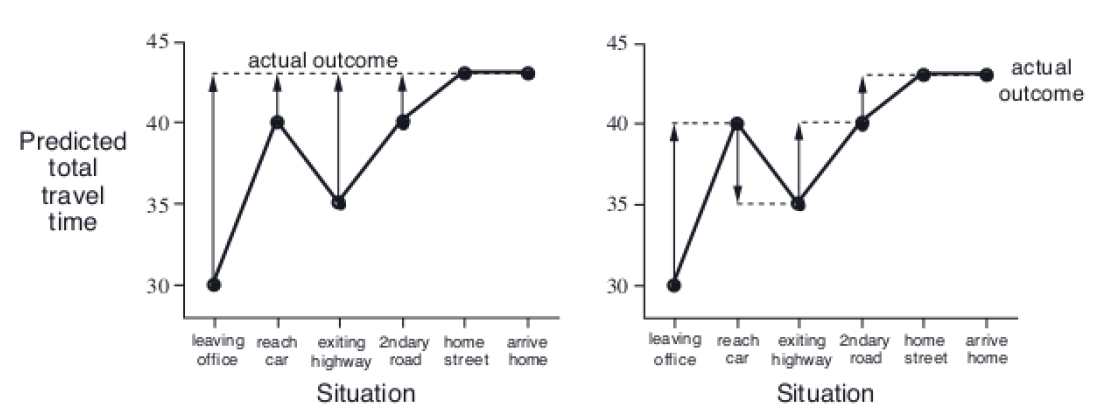
\includegraphics[width=1.0\textwidth]{mc_td}
  \caption{Porównanie aktualizacji funkcji wartości w przypadku metod Monte Carlo (po lewej) oraz metod TD (po prawej)}
\end{figure}

Metody w uczeniu ze wzmocnieniem dzielimy również ze względu na to czy ewaluacja polityki przebiega przy użyciu polityki, która została wykorzystana podczas generowania trajektorii. Metody ewaluujące tę samą politykę nazywamy \emph{on-policy}, natomiast te które działają na różnych politykach nazywamy \emph{off-policy}.

Dwoma podstawowymi algorytmami zaliczającymi się do TD learning jest \emph{SARSA (State-Action-Reward-State-Action} oraz \emph{Q-Learning}.

SARSA jest przykładem metody on-policy, która wykorzystuje funkcję wartości akcji, zamiast funkcji wartości stanu. W przypadku tej metody aktualizacja funkcji wartości akcji jest następująca:

$$ Q(S_t, A_t) \leftarrow Q(S_t, A_t) + \alpha \big[R_{t+1} + \gamma Q(S_{t+1}, A_{t+1}) - Q(S_t, A_t) \big] $$

Aktualizacja ta zachodzi dla każdego nieterminalnego stanu $S_t$, a w przypadku gdy $S_{t+1}$ jest terminalny, to $ Q(S_{t+1}, A_{t+1}) $ definiujemy jako zero. Cały proces zależny jest od piątki $ (S_t, A_t, R_{t+1}, S_{t+1}, A_{t+1}) $, skąd pochodzi nazwa algorytmu \emph{SARSA}.

Q-Learning natomiast jest przykładem metody off-policy, w której aktualizacja Q-funkcji przebiega następująco:

$$ Q(S_t, A_t) \leftarrow Q(S_t, A_t) + \alpha \big[R_{t+1} + \gamma \max_a Q(S_{t+1}, a) - Q(S_t, A_t) \big] $$

W ten sposób uczona się przez nas funkcja $Q$ bezpośrednio aproksymuje $Q_\ast$, niezależnie od tego jaka polityka jest przez nas wykorzystywana do wybierania kolejnych akcji.

\subsection{Rollout Algorithms}

Metody wykorzystujące model do podejmowania decyzji, nazywane metodami \emph{model-based}, opierają się na planowaniu kolejnych ruchów, które w przyszłości podejmie nasz agent. Główną metodą planowania jest \emph{planowanie w momencie podjęcia decyzji}, które skupia się na podejmowaniu decyzji po znalezieniu się w konkretnym stanie $S_t$, a więc wyborze akcji $A_t$. Najważniejszy dla nas wówczas jest stan, w którym się znaleźliśmy, mniej natomiast te odległe bądź już odwiedzone, do których już nigdy nie powrócimy. Niezwykle użyteczne okazują się one w przypadku gdy na podjęcie decyzji możemy poświęcić trochę czasu, jak np. w przypadku szachów czy Go, mniej przydatne będzie ono jeśli nasz program będzie musiał bardzo szybko podejmować decyzje. 

Algorytmy typu rollout są algorytmami planowania w momencie podjęcia decyzji  i bazują na bardzo podobnej zasadzie co metody Monte Carlo. Przybliżają one funkcję wartości akcji dla stanu, w którym się znajdują, za pomocą symulowania kolejnych trajektorii, podobnie jak w przypadku ewaluacji polityki w Monte Carlo. Ich celem jednak nie jest znalezienie optymalnej polityki $\pi_\ast$ czy też funkcji $q_\ast$, a zamiast tego służą nam do stworzenia \emph{rollout polityki} za każdym razem gdy znajdziemy się w jakimś stanie. Okazuje się że polityki otrzymane w ten sposób radzą sobie nadzwyczaj dobrze.

\subsection{Monte Carlo Tree Search}

Przeszukiwanie drzew metodą Monte Carlo, czyli \emph{Monte Carlo Tree Search (MCTS)} jest dość nowym podejściem w uczeniu ze wzmocnieniem, wykorzystanym między innymi w takich programach jak AlphaGo. 

MCTS jako algorytm rollout symuluje kolejne trajektorie rozpoczynające się w obecnym stanie, a kończące na stanie terminalnym. Rozszerza on ten pomysł poprzez przechowywanie i aktualizację funkcji wartości akcji dla kolejnych ruchów, zamiast jak to było w poprzednim przypadku, tylko dla stanu w którym się on znajduje. Tworzone jest wówczas drzewo, ukorzenione w obecnym stanie, które wraz z kolejnymi symulacjami się rozszerza i dokładniej aproksymuje Q funkcję. Dla stanów obecnych w drzewie, decyzję podejmujemy na podstawie funkcji wartości zawartej w węzłach drzewa, a politykę wytworzoną w ten sposób nazywamy \emph{polityką drzewa}. Gdy podczas symulowania trajektorii dochodzimy do liścia w naszym drzewie, to dalsza symulacja wykonywana jest na podstawie rollout polityki. Eksporacja zapewniona jest na poziomie polityki drzewa, na przykład za pomocą zastosowania polityki $\epsilon$-zachłannej.

Pojedyncza iteracja MCTS dzieli się na cztery kroki:

\begin{enumerate}
\item \textbf{Wybór.} Wybierane są kolejne stany należące do drzewa na podstawie polityki utworzonej z wartości funkcji akcji, która zdefiniowana jest przez krawędzie grafu. Przejście przez drzewo rozpoczyna się w korzeniu, a kończy w liściu drzewa.
\item \textbf{Rozwinięcie.} Drzewo jest rozszerzane w liściu, który został osiągnięty w poprzednim kroku, poprzez dodanie nowych węzłów jako dzieci dla tego liścia. Nowe węzły reprezentują stany, które wcześniej nie były obecne w drzewie.
\item \textbf{Symulacja.} Zaczynając w węźle wybranym w pierwszym punkcie, rozpoczynana jest symulacja na podstawie polityki rollout. W wyniku otrzymujemy trajektorię, której pierwsze ruchy zostały wybrane za pomocą polityki drzewa, a pozostałe -- polityki rollout.
\item \textbf{Propagacja wsteczna.} Wynik agenta jest propagowany wstecz do aktualizacji istniejących węzłów, bądź utworzenia nowych. Proces ten dotyczy jedynie stanów, które znajdują się w drzewie.
\end{enumerate}


\begin{figure}[ht!]
  \centering
  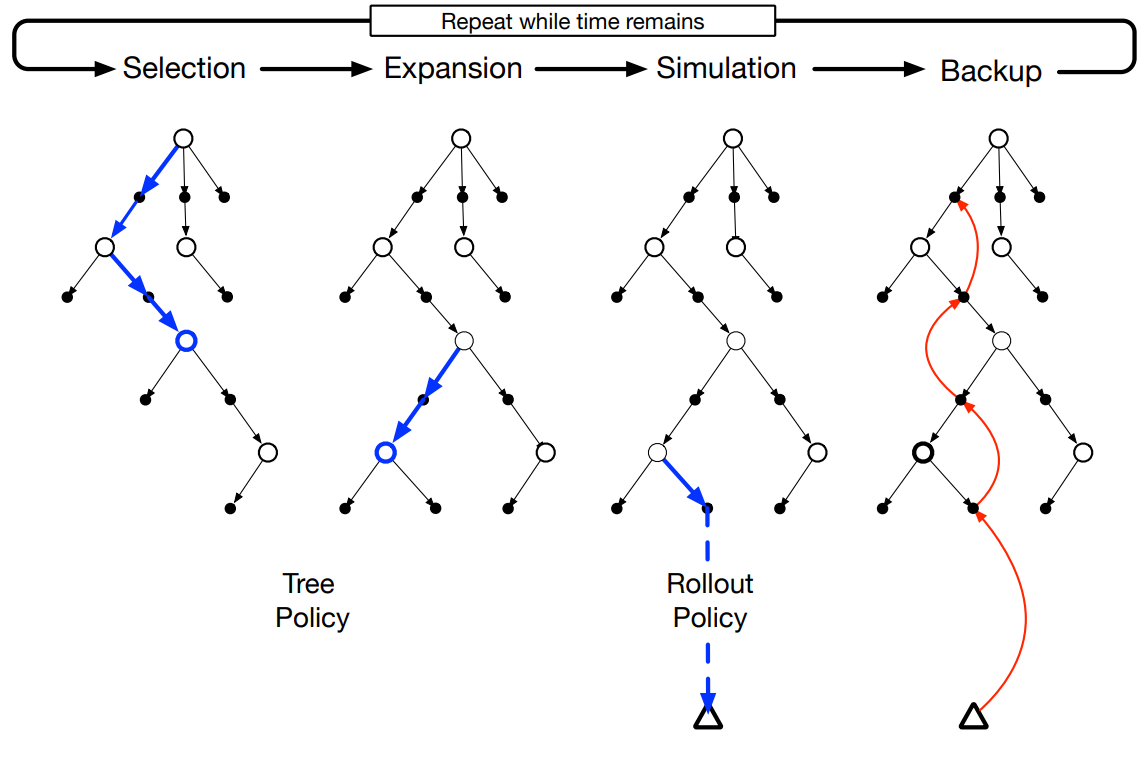
\includegraphics[width=0.85\textwidth]{mcts}
  \caption{Kolejne kroki podczas rozwijania drzewa w MCTS}
\end{figure}


\section{Podsumowanie}

W tym rozdziale zaprezentowane zostały podstawowe podejścia oraz koncepcje stosowane w uczeniu ze wzmocnieniem. Podczas tworzenia programów rozwiązujących gry strategiczne na planszy, jakimi są piłkarzyki na kartce czy Go, będziemy ze sobą łączyć te techniki, wzbogacając je dodatkowo o sieci neuronowe. W kolejnym rozdziale bliżej przyjrzymy się sieciom neuronowym, aby zrozumieć w jaki sposób one działają i jak możemy zastosować je do rozwiązania naszego problemu.

\chapter{Głębokie Sieci Neuronowe}

Ostatnio bardzo często mamy okazję słyszeć o Sztucznych Sieciach Neuronowych. Ponownie stały się one popularne wśród społeczności sztucznej inteligencji i obecnie osiągają najlepsze wyniki w bardzo wielu dziedzinach. Pozwalają nam one nam na tworzenie autonomicznych pojazdów, rozpoznawać obrazy lepiej od ludzi czy pokonać mistrza świata w Go. 

Głębokie Sieci Neuronowe mają zdolność do tworzenia aproksymacji nieliniowych funkcji na podstawie danych. Ponadto, w porównaniu do innych modeli uczenia maszynowego, nie wymagają one ręcznego tworzenia istotnych cech na podstawie danych, a zamiast tego same tworzą własną reprezentacje. Dzięki temu ograniczają one wymaganą interakcje z modelem, przy jednoczesnej poprawie jakości uzyskiwanych cech.

\section{Sieci jednokierunkowe}

Głębokie sieci jednokierunkowe (ang. Deep Feedforward Networks), zwane również wielowarstwowym perceptronem (ang. Multilayer Perceptron), są podstawowym modelem głebokiego uczenia. Ich zadaniem jest przybliżanie funkcji $ y = f^{\ast}(x) $, która dla danych wejściowych $x$ przyporządkowuje konkretną decyzję $y$ np. kategorię. Sieć jest wówczas funkcją $ y = f(x; \theta) $ parametryzowaną przez wektor $\theta$, który uczy się na podstawie danych.

Sieci neuronowe nazywane są sieciami, gdyż są one złożeniem wielu funkcji ze sobą, przez co informacje przepływają kolejno przez wszystkie z nich. Możemy je reprezentować jako acykliczny graf, który definiuje kolejne kroki wykonywanych obliczeń. Przykładowo możemy złożyć ze sobą dwie funkcje $ f(x) = f^{(2)}(f^{(1)}(x)) $, otrzymując sieć w której $f^{(1)} $ jest pierwszą warstwą sieci, a $ f^{(2)} $ -- drugą. Ilość składanych ze sobą sieci nazywamy \emph{głębokością} sieci, ostatnią warstwę -- \emph{warstwą wyjściową}, a pozostałe warstwy -- \emph{ukrytymi warstwami}. 

W sieciach jednokierunkowych przepływ informacji występuje w jednym kierunku, a więc każda z warstw jest zależna jedynie od poprzednich. Nie występuje w nich sprzężenie zwrotne, które jest charakterystyczne dla rekurencyjnych sieci neuronowych.

Sztuczne sieci neuronowe swoją budową bazują na prawdziwych sieci neuronowych, które występują w mózgu. Warstwy sieci scharakteryzowane są przez \emph{szerokość}, która mówi o rozmiarze wektora produkowanego przez odpowiadającą jej funkcję. Każdy element wektora może pełnić wówczas funkcję analogiczną do neurona, który zbiera wszystkie informacje z poprzedniego wektora i tworzy na ich podstawie pewną wartość. Wszystkie neurony w warstwie działają niezależnie od siebie. Pomimo jednak iż głębokie uczenie posiadają swoje korzenie w neuronaukach, to obecnie funkcje są dobierane przez inżynierów na podstawie ich własności matematycznych, a ich głównym celem nie jest już naśladowanie działania mózgu.

\section{Budowa neuronu}

Każdy z neuronów na wejściu przyjmuje wektor $x$, który odpowiada poprzedzającej mu warstwie. Następnie liczony jest jego iloczyn skalarny z wektorem wag $w$ i dodawane jest obciążenie $b$. Otrzymana wartość przekazywana jest do funkcji aktywacji $f$, a na końcu wyniki ze wszystkich neuronów są ze sobą konkatenowane w wektor, którego długość jest równa ilości neuronów w danej warstwie.

$$ y_i = f(\mathbf{x}^{T}\mathbf{w} + b) $$

Rolą funkcji aktywacji w sieciach neuronowych jest wprowadzenie nieliniowości do funkcji, dzięki którym możemy aproksymować dowolne funkcje. Najpopularniejszymi z nich są:

\begin{itemize}
\item Sigmoid:

$$ f(x) = \sigma(x) = \frac{1}{1 + e^{-x}}$$

\item Rectified Linear Unit (ReLU):

$$ f(x) = 
\begin{cases}
    x,              & \text{dla } x \geq 0\\
    0,              & \text{dla } x < 0
\end{cases}
$$

\item Tangens hiperboliczny:

$$ f(x) = \frac{e^x - e^{-x}}{e^x + e^{-x}} $$

\end{itemize}

W przypadku klasyfikacji, w której występuje wiele kategorii, wykorzystywana jest funkcja Softmax, która aplikowana jest od razu do całego wyjściowego wektora:


$$ f_i(x) = \frac{e^x}{\sum_j e^j} $$


\section{Uczenie sieci neuronowej}

Uczenie sieci neuronowej jest procesem optymalizacji, która polega na minimalizacji bądź maksymalizacji pewnej funkcji $ f(x; \theta) $ za pomocą zmieniania wartośći $ \theta $. Funkcja $ f $ jest przez nas nazywana \emph{funkcją celu}, w przypadku minimalizacji często nazywana jest również \emph{funkcją kosztu}, \emph{funkcją straty} lub \emph{funkcją błędu}. 

Optymalizacja przebiega przy użyciu gradientu funkcji $ f $. Znając jego wartość możemy zmodyfikować $\theta$ o niewielki krok $ \alpha $, zwany \emph{krokiem uczenia} (ang. learning rate), aby odpowiednio zmniejszyć bądź zwiększyć wartość funkcji $ f $. 

$$ \theta_{i+1} = \theta_i - \alpha f'(x; \theta_i) $$

Metoda ta nazywana jest \emph{metodą gradientu prostego} (ang. Stochastic Gradient Descent. SGD), a najczęściej stosowaną jej odmianą jest \emph{mini-batch SGD}, gdzie gradient liczony jest dla kilkudziesięciu przykładów z danych jednocześnie, po czym jest uśredniany. Przykłady pokazywane w jednym momencie sieci nazywane są \emph{partią} (ang. batch), a jedna iteracja w której siec widzi dokładnie wszystkie partie raz, nazywana jest epoką.

Podczas tworzenia modelu możemy natrafić na pojęcie \emph{parametrów} oraz \emph{hiperparametrów} sieci. Poprzez parametry sieci rozumiemy wektor cech $\theta$, który jest modyfikowany w procesie uczenia sieci, a wyznaczany on jest losowo. Hiperparametrami natomiast nazywamy te czynniki, które ręcznie wyznaczamy przed rozpoczęciem procesu uczenia i są one przez nas arbitralnie wybierane. Nie jest możliwe ich uczenie się przez algorytm, a ich dobór jest arbitralny. Przykładami hiperparametrów modelu mogą być takie rzeczy jak głębokość sieci, szerokość sieci, krok uczący czy rozmiar partii.

\begin{figure}[ht]
  \centering
  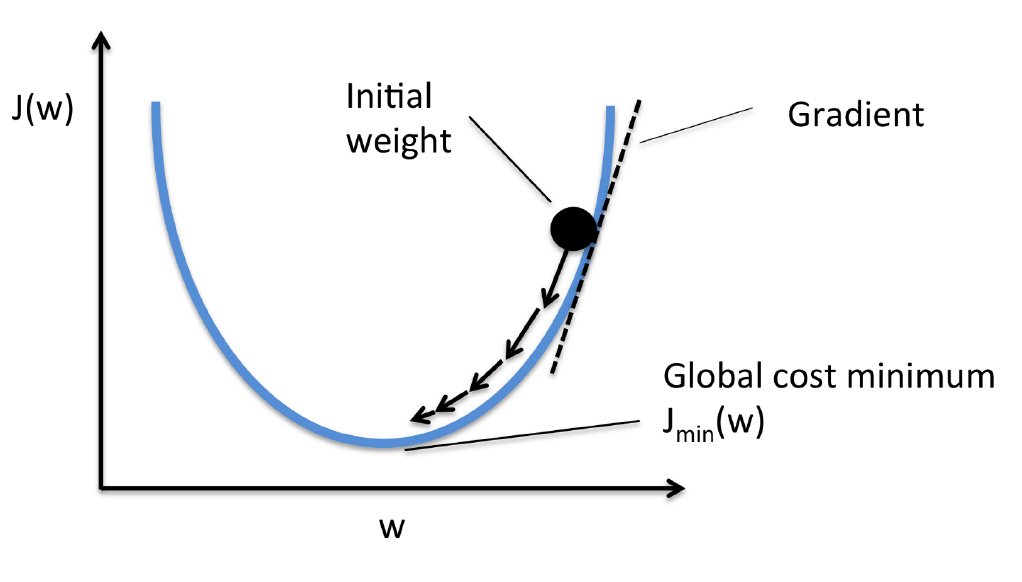
\includegraphics[width=0.5\textwidth]{sgd}
  \caption{Metoda stochastycznego gradientu prostego.}
\end{figure}

W zależności od rozwiązywanego przez nas zadania, dobiera się różne funkcje celu, a najpopularniejszymi z nich jest cross entropia (ang. Cross Entropy) w przypadku klasyfikacji:

$$ L_{log}(y, \hat{y}) = -\log\mathbb{P}(y | \hat{y}) = 
-\frac{1}{N} \sum_{i = 1}^N \sum_{k = 1}^M y_{i, k} \log \hat{y}_{i, k}
$$

gdzie $y$ to rzeczywista wartość funkcji, zwana również \emph{celem}, $\hat{y}$ to nasza predykcja, $N$ to rozmiar danych treningowych, a $M$ to liczba różnych klas. Dla modeli regresyjnych najczęściej wybieraną funkcją jest \emph{błąd średniokwadratowy} (ang. Mean Squared Error, MSE):

$$ L_{MSE}(y, \hat{y}) = \sum_{i = 1}^N (y_i - \hat{y}_i)^2$$

Różnica pomiędzy wykorzystaniem metod gradientowych optymalizacji w głębokim uczeniu maszynowym i klasycznym uczeniu maszynowym, jest fakt iż nieliniowość sieci neuronowych powoduje iż funkcje straty w większości przypadków nie są wypukłe. Z tego powodu zbieżność danych metod nie jest gwarantowana, a jakość otrzymanego modelu jest zależna od parametrów początkowych modelu. Powstało wiele metod aby unikać lokalne minima funkcji celu, a powszechnie stosowanymi oraz dającymi najlepsze rezultaty są obecnie \emph{Adam} oraz \emph{RMSprop}. 

\section{Propagacja wsteczna}

W celu wykonania predykcji przy użyciu naszego modelu, musimy przekazać mu przykład, dla którego utworzy on estymację. Informacja o nim zostaje przekazywana przez kolejne warstwy, aby ostatecznie zwrócić jakiś wynik. Każdy kolejny krok wykonywanych obliczeń możemy utożsamić z grafem, który definiuje w jaki sposób wygląda przepływ przez naszą sieć. Przetworzenie przykładu przez naszą sieć nazywamy wówczas \emph{propagacją} (ang. forward propagation). Otrzymana przez nas estymacja jest później wykorzystana w funkcji błędu. 

Algorytm propagacji wstecznej polega na przepływie sieci w przeciwnym kierunku, zaczynając od funkcji kosztu. Kolejne pochodne składające się na gradient liczone są przy pomocy metody łańcuchowej.

$$ \frac{dz}{dx} = \frac{dz}{dy} \frac{dy}{dx} $$
 

\section{Regularyzacja}

Częstym problemem występującym podczas uczenia sieci neuronowych oraz ogólnie modeli uczenia maszynowego jest problem zbytniego dopasowania do danych. Występuje on gdy funkcja błędu na zbiorze treningowym osiąga znacząco niższy poziom niż na zbiorze testowym, który nie był obecny podczas uczenia się sieci. Podejmowane są różne kroki w celu zmniejszenia różnicy pomiędzy błędami obserwowanymi na obu tych zbiorach, a najpopularniejszym i najprostszym z nich jest regularyzacja parametrów.

Regularyzacja parametrów wykorzystywana jest również w prostszych modelach statystycznych, takich jak regresja liniowa czy logistyczna. Zmniejsza ona teoretyczną pojemność modelu, co pozytywnie wpływa na jego jakość. Polega ona na dodaniu dodatkowego składnika do funkcji błędu, który odpowiada za zwiększanie jej wartości w zależności od parametrów sieci. Zmodyfikowana funkcja straty jest wówczas postaci:

$$ L'(y, \hat{y}) = L'(y, f(x; \theta)) = L(y, f(x; \theta)) + \alpha \Omega(\theta) $$, 

gdzie $ \Omega(\theta) $ jest pewną normą wektora $ \theta $. Najpopularniejszą wyborem jest norma $ L^2 $.

Innymi znanymi metodami regularyzacji są takie rzeczy jak augmentacja danych czy dropout.

\section{Normalizacja batchów}

Uczenie głębokich sieci neuronowych okazuje się bardzo trudnym zadaniem. Aktualizacje warstw następują jednocześnie dla całej sieci, natomiast same gradienty liczone są przy założeniu że pozostałe warstwy pozostaną takie same. Zmiana parametrów powoduje iż rozkład wartości dla każdej z warstw cały czas ulega zmianie, przez co musimy korzystać z małych learning rate, gdyż cały proces jest mocno niestabilny. Problem ten nazywany jest \emph{internal covariate shift} i rozwiązywany jest przez normalizację wyników z każdej warstwy. 

Normalizacja batchów (ang. Batch normalization) polega na reparametryzacji wyniku każdej z warstw, która wykonuje się przy każdej kolejnej propagacji partii. Po jej wykonaniu rozkład wartości z każdej z warstw ma zawsze tę samą średnią oraz wariancję.

$$ \mathbf{H'} = \frac{\mathbf{H} - \mathbf{\mu}}{\mathbf{\sigma}} $$

gdzie $ \mathbf{H} $ to wyjście z warstwy przed reparametryzacją, a $ \mathbf{H'} $ -- po reparametryzacji. Normalizacja batchów okazuje się również skuteczną metodą regularyzacji.

\section{Konwolucyjne Sieci Neuronowe}

\subsection{Wprowadzenie}

Konwolucyjne sieci neuronowe są specjalnym typem architektury sieci, które wykorzystują specyficzną topologię danych, które można reprezentować na pewnych kratach. Najpopularniejszym przykładem są zdjęcia, które można przedstawić jako 2-wymiarowe macierze pikseli oraz szeregi czasowe, które opisują pomiary oddalone od siebie jednakowymi interwałami czasowymi. Obecnie stanowią one state-of-the-art w wielu dziedzinach uczenia maszynowego, a w szczególności we wszelkich zadaniach związanych z wizją komputerową. 

\subsection{Operacja Konwolucji}

Konwolucyjne sieci swoją nazwę zawdzięczają matematycznej operacji konwolucji, która w naszym wypadku jest wykonywana na dyskretnych wartościach:

$$ s(t) = (x * w)(t) = \sum_{a = -\infty}^{\infty} x(a)w(t - a) $$

Standardową terminologią dla sieci konwolucyjnych jest określanie funkcji $x$ jako \emph{wejścia}, funkcji $w$ jako \emph{filtr} lub \emph{jądro}, a wynik operacji jako \emph{mapa cech}.

Często chcemy wykonywać operację konwolucji na wejściu o większej ilości wymiarów. W przpadku dwuwymiarowym wzór jest następujący:

$$ S(i, j) = (I * K)(i, j) = \sum_m \sum_n I(m, n) K(i - m, j - n) $$


\begin{figure}[ht!]
  \centering
  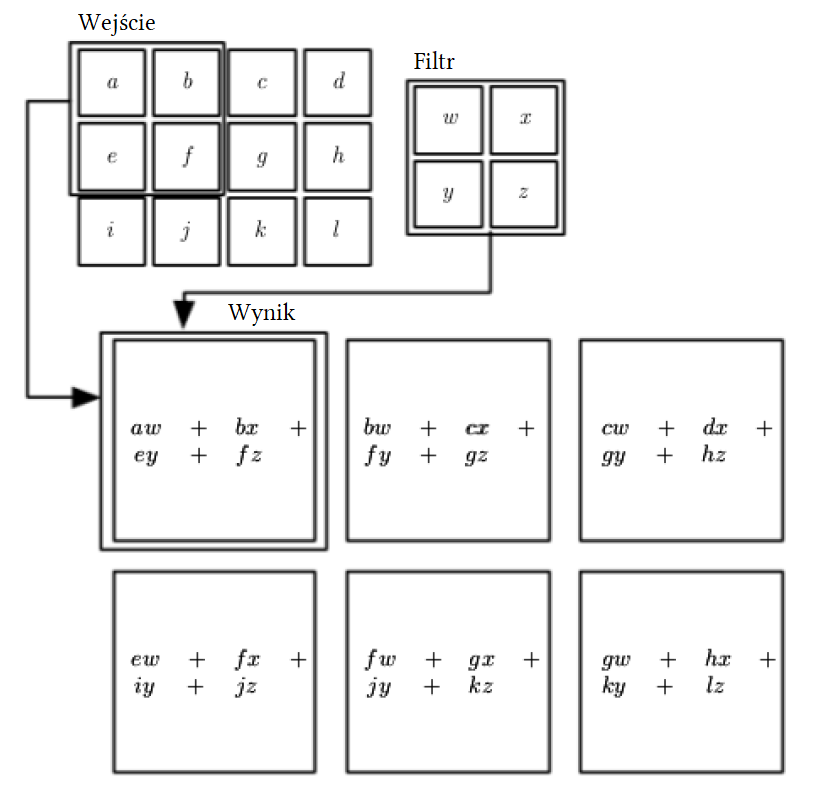
\includegraphics[width=0.85\textwidth]{konwolucja}
  \caption{Przykładowe wykonanie operacji konwolucji przy użyciu filtra 2 x 2}
\end{figure}

\subsection{Głębokie uczenie rezydualne}

Pogłębianie sieci neuronowych czyni je trudniejszymi do wyuczenia. Popularnym rozwiązaniem tego problemu jest wykorzystanie rezydualnych bloków, które umożliwiły trenowanie głębszych sieci, niż to było możliwe przed ich powstaniem. Obecnie wszystkie czołowe modele wykorzystywane podczas rozpoznawania obrazów wykorzystują tę architekturę.

Przypuśćmy że oczekiwanym przez nas mapowaniem z warstwy konwolucyjnej byłaby funkcja $ \mathcal{H}(x) $. Rezydalne mapowanie polega na tym, aby bezpośrednie wyjście z warstwy starało się dopasować do funkcji $ \mathcal{F}(x) = \mathcal{H}(x) - x $, po czym do niego jest dodawane $x$, uzyskując oczekiwaną wartość. Architektura ta okazuje się zdecydowanie poprawiać wyniki uczenia się sieci. Autorzy rezydualnego uczenia przypuszczają że sieciom neuronowym dużo łatwiej jest nauczyć się rezydualnego mapowania, zamiast tego standardowego. W skrajnym przypadku gdyby optymalnym mapowaniem była identyczność, to wówczas dużo łatwiej jest wyuczyć się przekształcenia o zerowym wyjściu, niż identyczności.

\begin{figure}[ht!]
  \centering
  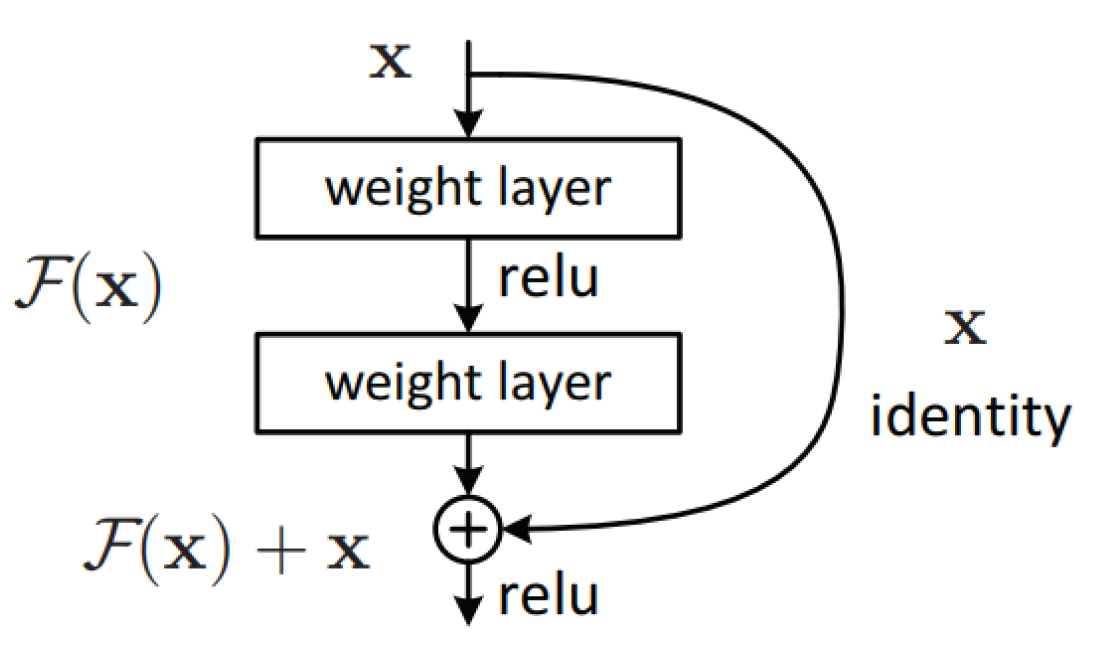
\includegraphics[width=0.6\textwidth]{res_block}
  \caption{Blok rezydualny}
\end{figure}

Rezydualne uczenie zazwyczaj jest aplikowane do kilku ustawionych po sobie warstw. Razem z połączeniem od wejścia nazywamy je blokiem budującym i definiujemy go jako:

$$ y = \mathcal{F}(x; \theta) + x $$.

Połączenie to nazywamy \emph{połączeniem skrótowym} (ang. shortcut connection). W przypadku gdy wymiar wejścia oraz wyjścia nie są sobie równe, to wykonujemy liniowe przekształcenie na wejściu, a blok definiujemy jako:

$$ y = \mathcal{F}(x; \theta) + W_sx $$,

gdzie $W_s$ to macierz wag odpowiadających za projekcje na wymiar wyjściowy.

\section{Podsumowanie}

Głębokie sieci neuronowe obecnie są najlepszym typem modeli do aproksymacji dowolnych funkcji, gdyż możemy je tworzyć jedynie na podstawie surowych danych i nie jest wymagane ręczne tworzenie cech ani nie jest potrzebna specjalistyczna wiedza z zakresu problemu, który staramy się przy ich użyciu rozwiązać. Z tego powodu są one również bardzo popularne wśród metod uczenia ze wzmocnieniem, jako przybliżenia funkcji wartości oraz polityki, a ich zastosowanie w tej dziedzinie zostanie opisane w kolejnym rozdziale.

\chapter{Głębokie Uczenie ze Wzmocnieniem}

\section{Wprowadzenie}

Obecnie uczenie ze wzmocnieniem w głównej mierze opiera się na wykorzystaniu sieci neuronowych jako aproksymatory funkcji wartości oraz polityki. Połączenie to pozwoliło nam na osiąganie niespotykanych dotąd wyników podczas rozwiązywania problemów takich jak gra w Dota 2 czy tworzenie autonomicznych samochodów. Dzięki zastosowaniu głębokiego uczenia jesteśmy w stanie radzić sobie z zadaniami, które charakteryzują się wielowymiarowością danych, a których rozwiązanie wcześniej było poza naszym zasięgiem.

Do głębokiego uczenia ze wzmocnieniem (ang. Deep Reinforcement Learning, DRL) zaliczamy takie metody jak \emph{głęboka Q-sieć} (ang. Deep Q-Network, DQN),  \emph{policy gradient} czy metody \emph{actor-critic}. Rozdział ten opisuje w jaki sposób te metody łączą się z sieciami neuronowymi, prowadząc do najskuteczniejszych obecnie algorytmów uczenia ze wzmocnieniem. 

\section{Deep Q-Learning}

Jednym z ważniejszych algorytmów ostatnich lat jest \emph{głęboka Q-sieć} (DQN), która jest połączeniem opisanego wcześniej \emph{Q-learningu} oraz konwolucyjnych sieci neuronowych. Autorzy wykorzystali ją do nauczenia agenta gry na Atari, gdzie bez zmiany hiperparametrów modelu, zastosowali go do 49 różnych gier osiągając w wielu z nich wyniki lepsze od ludzi. Przyjmowała ona na wejściu jedynie obraz w postaci macierzy pikseli oraz wynik uzyskiwany przez nią i na podstawie tych danych, bez dodatkowych interakcji, podejmowała decyzje.

W tym modelu sieć neuronowa pełni funkcję funkcji wartości akcji, tj. Q-funkcji, a podczas uczenia minimalizowana była następująca funkcja straty:

$$ L_i(\theta_i) = \mathbb{E}_{s \sim \rho_{\pi(\cdot)}, a \sim \pi(\cdot)} \Big[ (y_i^2 - Q(s, a; \theta_i))^2 \Big] $$

gdzie $ y_i = \mathbb{E}_{s' \sim \mathcal{E}'} \big[ r + \gamma \max_{a'} Q(s', a'; \theta_{i - 1}) \mid s, a \big] $ jest celem funkcji w $i$-tej iteracji, $\pi(s \mid a)$ jest polityką utworzoną na podstawie Q-funkcji, $\rho_{\pi(\cdot)} $ jest rozkładem stanów podczas podążania zgodnie z polityką $\pi$. Aktualizacja wag sieci następuje zgodnie z gradientem powyższej funkcji, który jest postaci:

$$ \nabla_{\theta_i}L_i(\theta_i) = \mathbb{E}_{s, a \sim p(\cdot); s' \sim \mathcal{E}} 
\Big[ \Big( r + \gamma \max_{a'} Q(s', a'; \theta_{i - 1}) - Q(s, a; \theta_i) \Big) \nabla_{\theta_i} Q(s, a; \theta_i) \Big] $$

Funkcja straty jest optymalizowana przy pomocy metody gradientu prostego. Jeżeli aktualizacje wag sieci następowałyby za każdym razem po zebraniu trajektorii, to mielibyśmy do czynienia z klasycznym algorytmem Q-learning. W odróżnieniu od uczenia z nadzorem, zamiast niezależnych danych treningowych, dostajemy próbki zależne od wag $\theta$ i z tego powodu musimy korzystać z dodatkowych metod, dzięki którym pozbywamy się silnej korelacji pomiędzy próbkami. Korzystamy z metody zwanej \emph{powtórkami z doświadczenia} (ang. experience replay), która polega na zebraniu wielu trajektorii podczas procesu interakcji agenta ze środowiskiem i zapisywaniu ich jako powtórki w pamięci, a następnie próbkowane są losowo konkretne przykłady $(s_t, a_t, r_{t+1}, s_{t+1})$. Zastosowanie tej techniki sprawia iż zmniejszana jest wariancja podczas procesu uczenia się, a sam agent szybciej i stabilniej osiąga satysfakcjonujące nas rezultaty.


\section{Policy Gradient}

Metody \emph{policy gradient} pozwalają nam na bezpośrednie modelowanie polityki agenta, bez konieczności korzystania z funkcji wartości. Możemy dzięki nim uzyskać politykę $\pi(a \mid s, \theta)$, która jest parametryzowana przez pewien wektor $\theta$. Proces optymalizacji utworzonej w ten sposób polityki polega na maksymalizacji pewnej \emph{funkcji nagrody}, którą otrzymuje nasz agent, za pomocą \emph{wzrostowej metody gradientu prostego} (ang. gradient ascent). W przeciwieństwie do standardowej funkcji błędu w głębokim uczeniu, którą zazwyczaj minimalizujemy, tym razem będziemy starać się maksymalizować funkcję nagrody.

Polityka może być dowolną funkcją $\pi(a \mid s, \theta)$, musi jednak być rózniczkowalna względem parametru $\theta$, abyśmy mogli wykorzystać metody gradientowe podczas jej uczenia. Uzyskana w ten sposób polityka jest stochastyczna, co w wielu przypadkach jest dla nas oczekiwanym efektem. Najczęstszym wyborem funkcji $\pi$ są sieci neuronowe, które znane są z innych dziedzin uczenia maszynowego. Aktualizacja parametrów naszego modelu może przebiegać zgodnie ze wzorem:

$$ \theta_{i+1} = \theta_i + \alpha \nabla_{\theta}J , \quad
J = \mathbb{E}_{\pi} \Big( \sum_{k = 0}^{\infty} \gamma^k r_k \Big)
$$

\section{Algorytm REINFORCE}

Najprostszym przykładem metody policy gradient jest algorytm \emph{REINFORCE}, który należy do metod Monte Carlo i opiera się na próbkowaniu kolejnych trajektorii przy użyciu polityki $\pi$, a następnie ulepszaniu jej na podstawie zebranego doświadczenia. \emph{Teoria Policy Gradient} daje nam przydatny wzór na proporcjonalność gradientu funkcji nagrody:

\begin{equation}\label{eq:pgt}
\nabla J(\theta) \propto \sum_s \mu(s) \sum_a q_{\pi} \nabla_{\theta} \pi(a \mid s, \theta)
\end{equation}

gdzie $\pi$ to polityka parametryzowana przez $\theta$, a $\mu$ jest \emph{rozkładem on-policy}, który mówi jaką część czasu spędzamy w każdym ze stanów. Formalnie definiujemy funkcję:

$$ \eta(s) = h(s) + \sum_{s'} \eta(s') \sum_{a} \pi(a \mid s') p(s \mid s', a) $$

gdzie $ h(s) $ oznacza prawdopodobieństwo rozpoczęcia się epizodu w stanie s, a zatem jest rozkładem początkowym stanów, a $p(s \mid s', a) $ jest prawdopodobieństwem przejścia ze stanu $s'$ do stanu $s$ po wykonaniu akcji $a$. Rozkład on-policy definiujemy wówczas jako:

$$ \mu (s) = \frac{\eta(s)}{\sum_s' \eta(s')} $$

Rozwijając dalej równanie \eqref{eq:pgt} otrzymujemy:

\begin{align*}
\nabla J(\theta) \propto & \sum_s \mu(s) \sum_a q_{\pi} \nabla_{\theta} \pi(a \mid s, \theta) \\
= & \mathbb{E}_\pi \Bigg[ \sum_{a} q_\pi (S_t, a) \nabla_\theta \pi(a \mid S_t, \theta) \Bigg]
\end{align*}

i w ten sposób pozbywamy się rozkładu $\mu$, który w przeciwnym wypadku musielibyśmy modelować lub znać. Zauważmy również że w tym wypadku wystarcza nam proporcjonalność tego wyrażenia, gdyż aktualizacje parametrów będą wykonywane o pewien arbitralnie dobrany krok uczący $\alpha$, który jest w stanie zniwelować wszelkie stałe nieproporcjonalności. Wykonując kolejne rachunki otrzymujemy: 

\begin{align*}
\nabla J(\theta) \propto  & \mathbb{E}_\pi \Bigg[ \sum_{a} \pi(a \mid S_t, \theta) q_\pi (S_t, a) \frac{\nabla_\theta \pi(a \mid S_t, \theta)}{\pi(a \mid S_t, \theta)} \Bigg] \\
= & \mathbb{E}_\pi \Bigg[ q_\pi(S_t, A_t) \frac{\nabla_\theta \pi(A_t \mid S_t, \theta)}{\pi(A_t \mid S_t, \theta)} \Bigg] \\ 
= & \mathbb{E}_\pi \Bigg[ G_t \frac{\nabla_\theta \pi(A_t \mid S_t, \theta)}{\pi(A_t \mid S_t, \theta)} \Bigg] 
\end{align*}

zamieniając w pierwszym przejściu $a$ na obserwację $A_t \sim \pi$, a następnie korzystamy z własności $ \mathbb{E}_\pi \big[ G_t \mid S_t, A_t \big] = q_\pi(S_t, A_t) \big] $. W ten sposób otrzymujemy wyrażenie, które możemy wykorzystać podczas próbkowania kolejnych trajektorii do aktualizacji parametrów naszej sieci.

$$ \theta_{t+1} = \theta_t + \alpha G_t \frac{\nabla_\theta \pi(A_t \mid S_t, \theta)}{\pi(A_t \mid S_t, \theta)} $$

Często możemy również spotkać się z innym zapisem wyrażenia $  \frac{\nabla_\theta \pi(A_t \mid S_t, \theta)}{\pi(A_t \mid S_t, \theta)}$:

$$  \frac{\nabla_\theta \pi(A_t \mid S_t, \theta)}{\pi(A_t \mid S_t, \theta)} = \nabla_\theta \ln \pi(A_t \mid S_t, \theta) $$

Metoda REINFORCE może zostać wzbogacona o \emph{wartości bazowe} $b(s)$:

$$ \nabla J(\theta) \propto \sum_s \mu(s) \sum_a \Big( q_\pi(s, a) - b(s) \Big) \nabla_\theta \pi(a \mid s, \theta) $$,

których celem jest ograniczenie wariancji podczas uczenia się modelu. Warunkiem który funkcja $b$ musi spełniać jest jej niezależność od $a$, gdyż wtedy nie wprowadza ona dodatkowego obciążenia:

$$ \sum_a b(s) \nabla_\theta \pi(a \mid s, \theta) = b(s) \nabla_\theta \sum_a \pi(a \mid s, \theta) = b(s) \nabla_\theta 1 = 0 $$

Aktualizacja wag przyjmuje wówczas postać:

$$ \theta_{t+1} = \theta_t + \alpha \Big( G_t - b(S_t) \Big) \frac{\nabla_\theta \pi(A_t \mid S_t, \theta)}{\pi(A_t \mid S_t, \theta)} $$


Algorytm REINFORCE, podobnie jak wszystkie metody Monte Carlo, uczy się bardzo wolno, gdyż estymacje obarczone są wysoką wariancją. Rozwiązaniem tej niedogodności okazują się być modele przedstawione w kolejnej sekcji.

\section{Metody Aktor Krytyk}

Metody aktor krytyk są połączeniem modeli bazujących na modelowaniu polityki oraz tych bazujących na funkcji wartości. Polityka w tych metodach nazywana jest \emph{aktorem}, gdyż odpowiada ona za podejmowanie wykonywanych decyzji. Funkcja wartości nazywana jest \emph{krytykiem} i jej rolą jest ocenianie jakości akcji wykonywanych przez aktora. Parametry polityki są wówczas aktualizowane na podstawie estymacji wykonanych przez aktora.

Jednym z prostszych algorytmów, który można przytoczyć jako przykład, jest jednokrokowa metoda aktor krytyk, która koncepcyjnie jest bardzo podobna do takich algorytmów jak TD(0) czy Sarsa. Pozwala ona na w pełni online algorytm uczenia, w którym wynik z pełnej trajektorii $G_t$ zamieniany jest na wynik jednokrokowy:

\begin{align*}
\theta_{t+1} =& \theta_t + \alpha \Big( G_t - \hat{v}(S_t, w) \Big) \frac{\nabla_\theta \pi(A_t \mid S_t, \theta)}{\pi(A_t \mid S_t, \theta)} \\
=& \theta_t + \alpha \Big( R_{t+1} + \gamma \hat{v}(S_{t+1}, w) - \hat{v}(S_t, w) \Big) \frac{\nabla_\theta \pi(A_t \mid S_t, \theta)}{\pi(A_t \mid S_t, \theta)} \\
=& \theta_t + \alpha \delta \frac{\nabla_\theta \pi(A_t \mid S_t, \theta)}{\pi(A_t \mid S_t, \theta)}
\end{align*}

gdzie $ \hat{v}(S_t, w) $ jest aproksymowaną funkcją wartości stanu, parametryzowaną przez wektor $w$, a $\delta$ jest TD-błędem. Funkcja wartości dla stanu $S_t$ jest początkowo odejmowana od wyniku $G_t$ jako wartość bazowa. 

\section{Podsumowanie}

Dla większości obecnie rozwiązywanych problemów przy użyciu uczenia ze wzmocnieniem, to modele głębokiego uczenia są poziomem state-of-the-art i to na nich skupiona jest obecnie największa uwaga. W przypadku algorytmu AlphaGo Zero jego autorzy poszli o kolejny krok do przodu, włączając do modelu również przeszukiwanie drzewa rozgrywki, osiągając tym samym rezultaty które wcześniej wydawały się niemożliwe do uzyskania. Rozszerzenie tych metod zostanie opisane w kolejnym rozdziale, gdzie wykorzystując algorytm AlphaGo Zero staram się rozwiązać problem gry w piłkarzyki na papierze.

\chapter{Gra w piłkarzyki na kartce}

\section{Wprowadzenie}

Wielu specjalistów od dawna zajmuje się tworzeniem systemów grających w gry planszowe. Pierwszym krokiem milowym w rozwoju inteligentnych systemów było utworzenie Deep Blue, algorytmu potrafiącego grać w szachy, który w 1997 pokonał ówczesnego mistrza świata Garrego Kasparowa. Kolejnym celem stało się wówczas rozwiązania gry w Go, w której ilość ruchów na każdą rundę oraz długość rozgrywki są nieporównywalnie większe niż w przypadku szachów. W ostatnim czasie zespołowi z Deep Mind udało się utworzyć algorytm AlphaGo, który w roku 2016 pokonał mistrza świata Lee Sedol'a. Łączył on wszystkie znane do tamtej pory techniki wykorzystywane w uczeniu ze wzmocnieniem oraz głębokie uczenie, a w ubiegłym roku, 2017, został on rozwinięty algorytmu AlphaGo Zero, który zupełnie generycznie, bez jakiejkolwiek wiedzy specjalistycznej, wykorzystując jedynie plansze jako wejście, osiągnął ponadludzkie zdolności gry w Go, wygrywając wszystkie gry przeciw wcześniejszemu algorytmowi. 

Algorytm uczący agenta grającego w piłkarzyki na papierze jest w całości oparty na algorytmie AlphaGo Zero. Zmodyfikowana została jedynie architektura sieci oraz hiperparametry wykorzystane podczas uczenia.

\section{Metoda uczenia poprzez grę z samym sobą}

Iteracja polityki jest procesem w którym naprzemiennie wykonywana jest estymacja funkcji wartości na podstawie posiadanej polityki oraz ulepszanie obecnej polityki. Może się to odbywać przykładowo za pomocą próbkowania kolejnych trajektorii w pierwszym przypadku, a w drugim poprzez zamianę polityki na zachłanną względem otrzymanej funkcji wartości.

Lepszym pomysłem, wykorzystywanym w \emph{classification-based} uczeniu ze wzmocnieniem, jest wykorzystanie metod przeszukiwania drzew Monte Carlo. Próbkujemy w nich wiele trajektorii przed wykonaniem każdej z akcji i wybieramy tę akcję, która przyniosła najlepsze rezultaty podczas próbkowania, a następnie wybrana akcja służy jako pozytywny przykład uczący, a pozostałe jako negatywne.

W przypadku AlphaGo Zero tworzona jest polityka drzewa, na której podstawie wybierane są akcje, a następnie podstawowa polityka jest ulepszana na podstawie uprzednio otrzymanego rozkładu prawdopodobieństwa. Polityka drzewa tworzona jest na podstawie podstawowej polityki oraz funkcji wartości, które przechowywane są jako głęboka sieć neuronowa.

Polityka oraz funkcja wartości są głęboką sieć neuronowa $f_\theta$, która przyjmuje na wejściu obecny stan gry, a produkuje w wyniku rozkład prawdopodobieństw po wszystkich możliwych akcjach oraz funkcję wartości dla tego stanu, $f_\theta(s) = (p, v)$.

\subsection{Rozgrywanie gier}

Przez cały czas trwania algorytmu przechowywany jest najlepszy gracz $\alpha_{\theta^\ast}$, który wykorzystywany jest do generowania przykładów uczących. Rozgrywa on kolejne gry między sobą, zapisując przebieg oraz wynik każdego z meczów, jako ciąg wszystkich wykonanych akcji $(s_t, \pi_t, r_t)$, gdzie $s_t$ to stan gry, $\pi_t$ to rozkład akcji z polityki drzewa, a $r_t$ to zwycięzca gry. Wszystkie te wartości są z perspektywy gracza wykonującego ruch w czasie $t$.

\subsection{Trenowanie na zebranym doświadczeniu}

Po zakończonej fazie rozgrywania gier, rozpoczynane jest trenowanie sieci. W tym celu losowane są przykłady z wykonanych akcji, a następnie optymalizowana następująca funkcja straty:

$$ (p, v) = f_\theta(s) \quad
L = (r - v)^2 - \pi^T \log p + c \lvert \lvert \theta \rvert \rvert^2
$$

gdzie $c$ jest współczynnikiem regularyzacyjnym.	

\subsection{Ewaluacja wyuczonej polityki}

W trakcie uczenia się sieci, co pewien czas wykonywana jest ewaluacja wytrenowanego agenta, która polega na rozegraniu pewnej ilości gier pomiędzy nim a najlepszym graczem $\alpha_{\theta^\ast}$. W przypadku gdy stosunek gier wygranych przez nowego agenta przekroczy ustalony poziom, wynoszący 55\%, to staje się on nowym najlepszym graczem, a dalszy trening jest przerywany i rozpoczynana jest kolejna epoka.

\section{Algorytm przeszukujący drzewo gry}

Akcje podejmowane podczas rozgrywki są oparte na polityce drzewa, która budowana jest w trakcie rozgrywki. Wykorzystywany jest do tego algorytm MCTS, opierający się na wynikach z sieci neuronowej. Krawędzie w drzewie, które odpowiadają parze $(s, a)$ -- stan, akcja, przechowują wartości o prawdopodobieństwie wyboru tej akcji przy obecnej polityce $P(s, a)$, licznik odwiedzin $N(s,a)$ oraz funkcję wartości akcji $Q(s,a)$. Wykorzystanie MCTS intuicyjnie może być rozumiane jako algorytm do gry z samym sobą, gdyż przed wykonaniem ruchu nasz agent wykonuje szereg symulacji i na ich podstawie dokonuje decyzji. 

\subsection{Wybór ścieżki w drzewie}

Wybór akcji rozpoczyna się w korzeniu drzewa gry, który reprezentuje rzeczywisty stan, w którym znajduje się agent. Wykonywane są kolejne symulacje, które polegają na wykonywaniu kolejnych akcji, aż agent natrafi na liść. Wówczas wykonywane jest rozwinięcie danego liścia do nowego węzła i jego ewaluacja. Symulacje wykorzystują statystyki $\big(N(s,a), W(s,a), Q(s,a), P(s,a) \big)$, gdzie $N, Q, P$ są takie jak w poprzednim podpunkcie, a $W(s,a)$ jest sumą do tej pory zaobserwowanych funkcji wartości. Akcjami wykonywanymi w kolejnych krokach są $a_t = \operatorname*{argmax}_a \big( Q(s_t, a) + U(s_t, a) \big)$, gdzie $U$ zdefiniowane jest następująco:

$$ U(s,a) = c_{puct} P(s,a) \frac{\sqrt[]{\sum_b N(s,b)}}{1 + N(s,a)} $$

gdzie $c_{puct}$ jest to stała wyznaczająca poziom eksploracji podczas symulacji. W ten sposób początkowo zapewniona jest eksploracja, gdyż najpierw wybierane są akcje z wysokim początkowym prawdopodobieństwem, ostatecznie jednak preferowane są akcje z wysoką wartością funkcji wartości akcji.

\subsection{Rozwinięcie i ewaluacja nowego węzła}



\subsection{Propagacja wsteczna}

\subsection{Wybór akcji}

\section{Pierwsze testy na zmniejszonej planszy}

\section{Wyniki dla gry standardowych rozmiarów}

\section{Podsumowanie}

\chapter{Wnioski}

\begin{thebibliography}{99}

\end{thebibliography}

\end{document}


%%% Local Variables:
%%% mode: latex
%%% TeX-master: t
%%% coding: latin-2
%%% End:
